\documentclass[8pt]{beamer}

\usepackage{amsfonts}
\usepackage{subfiles}
\usepackage[T2A]{fontenc}
\usepackage[utf8]{inputenc}
\usepackage[russian]{babel}

\usepackage{amsmath, amsfonts, amssymb, amsthm, mathtools, mathrsfs}
\usepackage{wasysym, dsfont}
\usepackage{graphicx}
\usepackage{float}
\usepackage{wrapfig}

\usepackage{caption}
\usepackage{subcaption}
\usepackage{longtable}
% \usepackage{subfigure}

\usepackage{multicol}
\DeclareMathOperator*{\argmax}{\arg\!\max}
\DeclareMathOperator*{\argmin}{\arg\!\min}

\mode<presentation>
{
	\usetheme{boxes}
	\beamertemplatenavigationsymbolsempty
	
	\setbeamertemplate{footline}[page number]
	\setbeamersize{text margin left=1.5em, text margin right=2.0em}
}
\newcommand\blfootnote[1]{%
	\begingroup
	\renewcommand\thefootnote{}\footnote{#1}%
	\addtocounter{footnote}{-1}%
	\endgroup
}
\newcommand\FontUP{\fontsize{12}{14}\selectfont}


\title[]{Применение Neural-ODE для некоторых простых уравнений с особыми точками}
\author{Охотников Никита Владимирович}
\institute{МФТИ}
\date{2023}

\begin{document}

{
\begin{frame}
  \titlepage
\end{frame}
}

\begin{frame}
	\FontUP
	\frametitle{Постановка задачи}
	\begin{columns}
		\begin{column}{0.9\textwidth}
	
			\begin{block}{Цель}
				\smallskip
			Исследовать возможности приближения динамики дифференциальных уравнений с особыми точками  с помощью полносвязной нейронной сети
			\end{block}	
			\vfill
			\begin{block}{Предлагается}
				\smallskip
				Сравнить истинное поле касательных к графику решения и полученное с помощью Neural-ODE
			\end{block}	
			\vfill
			\begin{block}{Рассматриваемые уравнения}
				\smallskip
				$$y' = \frac{y}{x},~~~~y' = -\frac{y}{x},~~~~y' = -\frac{x}{y},~~~~y' = \frac{(x+y)}{(x-y)}$$
			\end{block}	
	     \end{column}
	\end{columns}
\end{frame}


\begin{frame}
	\FontUP
	\frametitle{Постановка задачи}
	\begin{columns}
		\begin{column}{0.9\textwidth}
			
			\begin{block}{Преобразование уравнений}
				\smallskip
				$$y' = \frac{y}{x} ~~~\xrightarrow{\hspace*{2cm}}~~~ \begin{cases} \dot{x} = -x \\ \dot{y} = -y
					\end{cases}$$
				$$y' = -\frac{y}{x}~~~\xrightarrow{\hspace*{2cm}}~~~ \begin{cases} \dot{x} = -x \\ \dot{y} = y
				\end{cases}$$
				$$y' = -\frac{x}{y}~~~\xrightarrow{\hspace*{2cm}}~~~ \begin{cases} \dot{x} = y \\ \dot{y} = -x
				\end{cases}$$
				$$y' = \frac{(x+y)}{(x-y)}~~~\xrightarrow{\hspace*{2cm}}~~~ \begin{cases} \dot{x} = y-x \\ \dot{y} = -y-x
				\end{cases}$$
			\end{block}	
		\end{column}
	\end{columns}
\end{frame}


\begin{frame}
	\frametitle{Результаты экспериментов}
	\begin{center}
		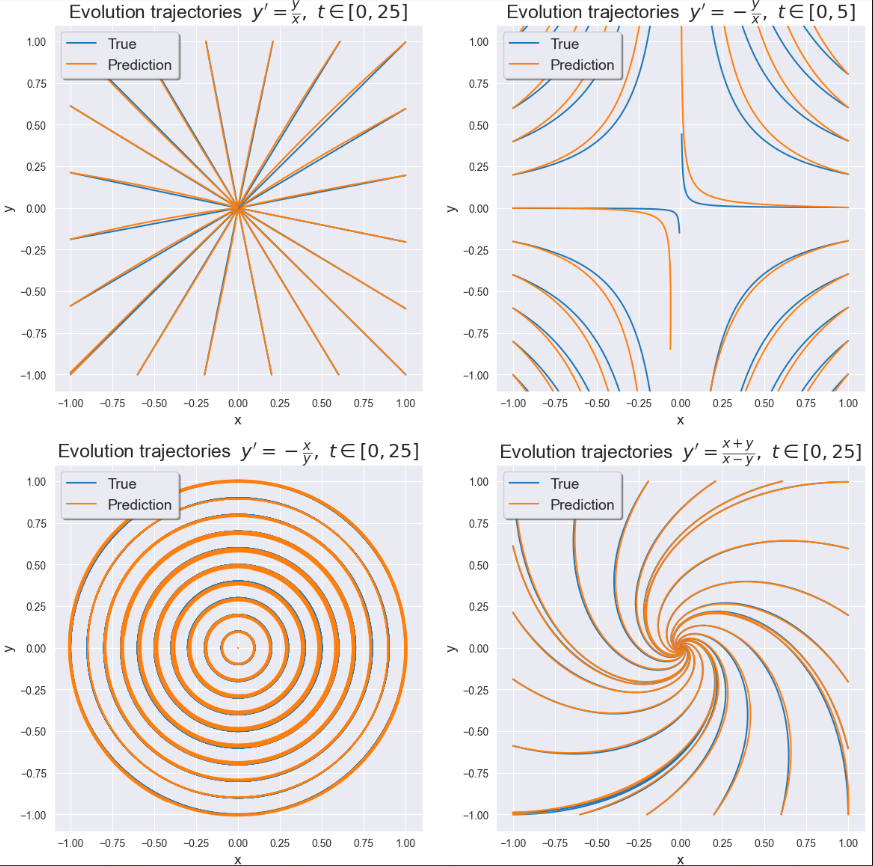
\includegraphics[scale = 0.37]{trajectories.png}
	\end{center}
\end{frame}

\begin{frame}
	\frametitle{Результаты экспериментов}
	\begin{center}		
		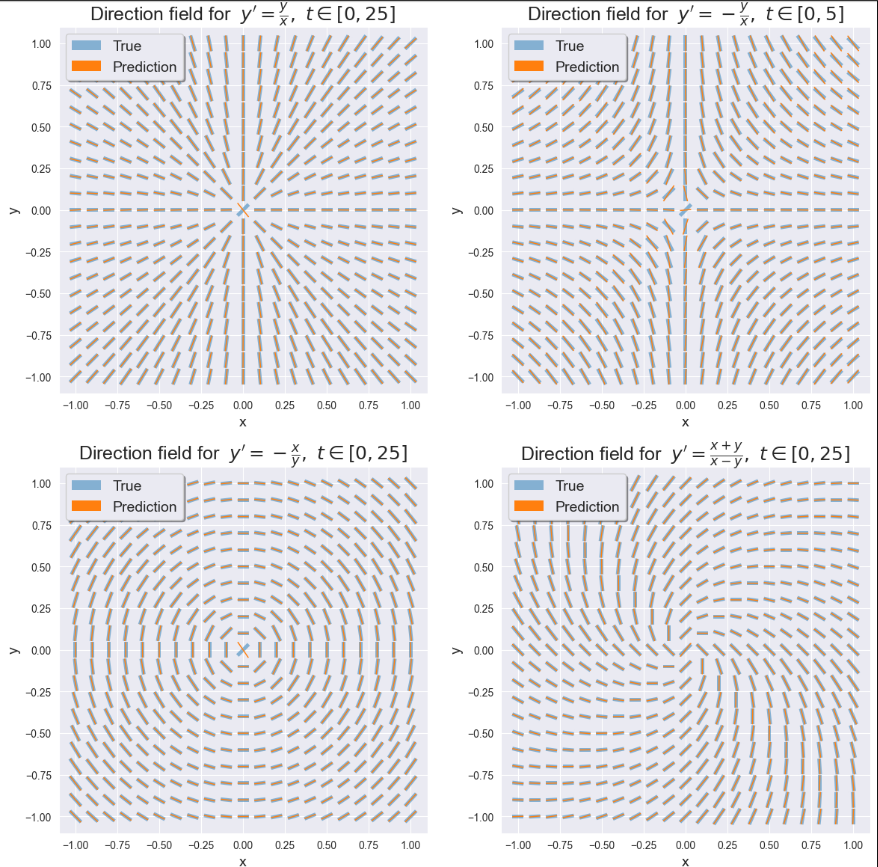
\includegraphics[scale = 0.37]{direction field.png}
	\end{center}
\end{frame}

\begin{frame}
	\frametitle{Результаты экспериментов}
	\begin{block}{Без параметризации через t}
		\begin{columns}
			\begin{column}{0.5\textwidth}
				\begin{center}
					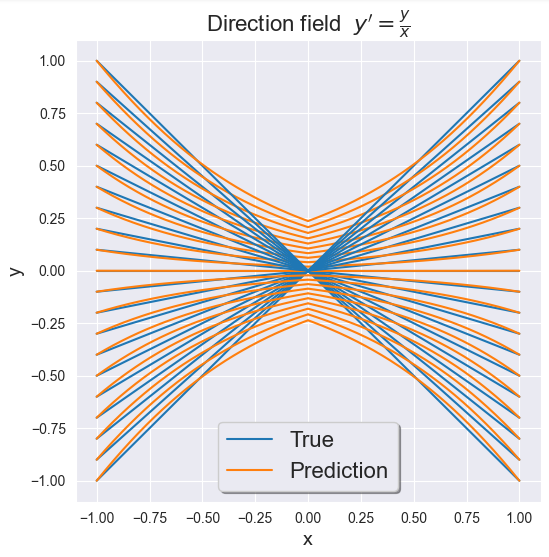
\includegraphics[scale = 0.37]{bad_uniform.png}
				\end{center}				
			\end{column}
			\begin{column}{0.5\textwidth}
				\begin{center}
					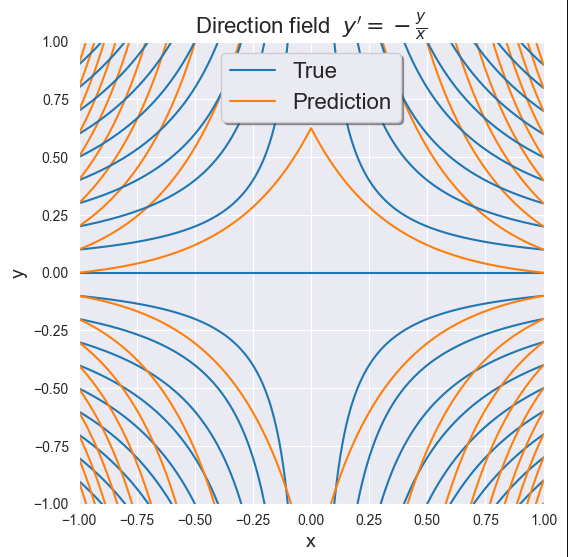
\includegraphics[scale = 0.37]{bad_saddle.png}
				\end{center}
			\end{column}
		\end{columns}
	Решения оставшихся двух уравнений не выражаются явной функцией $y = f(x)$ поэтому для них в любом случае необходима параметризация. 
	\end{block}

\end{frame}

\begin{frame}
	\frametitle{Выводы}
	\FontUP
	\begin{itemize}
		\item Рассмотрено решение дифференциальных уравнений вблизи особых точек с помощью Neural-ODE
		\vfill
		\item Найдена проблема с вертикальными асимптотами
		\vfill
		\item Показана неоправданность отказа от параметризации через дополнительный параметр -- время.
	\end{itemize}		
\end{frame}


\end{document}
